% Tutorial 01

\subsection{Tutorial 1: $S^2$ order parameter restraining}
The backbone N-H order parameter is a measure for the spatial restriction that the N-H vector experiences in a molecular reference frame. 
Order parameters calculated from ensembles generated by MD simulations are not subject to a specific motional model but depend on the 
local flexibility inherent in the force field when solving Newton's equation of motion and on whether the assumption of internal motion 
being independent of overall tumbling is justified. 
GROMOS features a time-averaging variant of order parameter restraining that is described in detail elsewhere \cite{Hansen_S2_2014}. 
Such time-averaged restraining enhances the configurational sampling by forcing the molecule to surmount barriers that would, without restraining, only be surmounted rarely, 
that is, on longer time-scales. Moreover, a possible force-field deficiency hampering the agreement with experiment can be redressed using this restraining technique. 
In this way configurational ensembles consistent with NMR data can be generated allowing a structural interpretation of experimental observations \cite{Smith_2017,Smith_2021}.
We will demonstrate the use of time-averaged order parameters by means of the third IgG-binding domain of Protein G (GB3), which is a small 56-residue protein.

\subsubsection{Topology}
%\textcolor{green}{Should we always provide a list of input files in each subsection as well as a list of generated output files? Or should we point to vol7 for this fine structure?}
Go into the subdirectory \texttt{topo} of the directory \texttt{t\_01}. The input file \texttt{make\_top\_GB3.arg} is already prepared. We will use the force field 54a7. 
The molecular topology file for the protein, \texttt{GB3\_54a7.top}, with SPC water as a solvent can then be generated using the GROMOS++ program \texttt{make\_top} 
by typing
\begin{lstlisting}
$ make_top @f make_top_GB3.arg > GB3_54a7.top
\end{lstlisting}
In order to neutralize the net charge of -2e of the protein topology the next step is to build a topology file for a sodium ion using the input file \texttt{make\_top\_Na.arg}:
\begin{lstlisting}
$ make_top @f make_top_Na.arg > Na_54a7.top
\end{lstlisting}
Next we combine the two topologies using the GROMOS++ program \texttt{com\_top}
\begin{lstlisting}
$ com_top @f com_top_GB3_2Na.arg > GB3_2Na_54a7.top
\end{lstlisting}
The file \texttt{GB3\_2Na\_54a7.top} contains the complete molecular topology. Using the GROMOS++ program \texttt{check\_top} with the arguments \texttt{@build} and \texttt{@param} the topology can be checked against the force field. 
The 34 types of logical checks performed are listed in volume 5 of the documentation \cite{volume_5}.
Be aware that \texttt{check\_top} may not catch every inconsistency 
or that an inconsistency pointed out by \texttt{check\_top} may not necessarily indicate an error in the topology.
In the present case the putative inconsistency with the partial charge on atom 5 spotted by \texttt{check\_top} is 
actually not an error because the partial charge is adapted for the N-terminus of the peptide chain.
Therefore, it is important to assure oneself that the topology generated is the one intended.

\subsubsection{Coordinates}

Go into the subdirectory \texttt{coord}. The Cartesian coordinates for the protein can be downloaded from the Protein Databank, accession code 2OED \cite{Ulmer_2003}. By using the GROMOS++ program \texttt{pdb2g96} the PDB file will be converted to a GROMOS coordinate file. Before conversion we make a copy of the downloaded pdb file \texttt{2oed.pdb} into the file \texttt{2oed\_edited.pdb}. In the latter we do a change in line 1010 (replace “O~” by “O1”) and line 1016 (replace “OXT” by “O2~”) such that \texttt{pdb2g96} recognizes these two atoms as belonging to the carboxy terminus. When editing the PDB file the columns must be kept aligned. The remaining differences between the nomenclature used in the PDB file and the one used in the topology are handled via the file \texttt{pdb2g96.lib}. With
\begin{lstlisting}
$ pdb2g96 @f pdb2g96_GB3.arg > pdb2g96_GB3.cnf
\end{lstlisting}
we generate a GROMOS coordinate file. 
Since the used NMR structure contains more hydrogen atoms than needed by the united-atom GROMOS force field, merging aliphatic hydrogen and carbon atoms into one interaction site, 
a list of warnings regarding ignored hydrogen atoms is issued, which can be ignored. If the initial structure was determined using X-ray diffraction, missing hydrogen atoms can be generated 
with the GROMOS program \texttt{gch} as explained in the basic tutorial.

\subsubsection{Energy minimization}

Before putting the protein in a box of solvent, its configuration is relaxed by energy minimization 
in vacuo to release possible strain induced by small differences in bond lengths, bond angles, improper dihedral angles and short non-bonded contacts 
between the force-field parameters and the NMR structure.
Go into the subdirectory \texttt{min} and open the shell script \texttt{em\_GB3.run} to adapt the paths and the names of the files according to your system. 
The energy minimization of the solute in vacuo is very fast and can be run interactively by typing
\begin{lstlisting}
$ ./em_GB3.run
\end{lstlisting}
Once the energy minimization is finished the minimized coordinates are written to the file \texttt{GB3\_min.cnf} and the general output file \texttt{em\_GB3.omd} contains the progress of the minimization.

\subsubsection{Solvating the protein in a water box}

Now the protein is ready to be placed into a box and solvated for subsequent simulations under periodic boundary conditions. Go into the subdirectory \texttt{box}. The box shape will be chosen to be rectangular, the simple point charge (SPC) water model \cite{Berendsen1981} will be employed (as already specified in the topology file), the minimum solute-to-wall distance will be 1.2 nm such that the closest surface atoms of two periodic copies are at least 2.4 nm apart (longer than the cutoff distance of 1.4 nm). The minimum solute-solvent distance is set to 0.23 nm. The GROMOS++ program \texttt{sim\_box} is used to generate the box and to solvate the protein by executing
\begin{lstlisting}
$ sim_box @f sim_box_GB3.arg > sim_box_GB3.cnf
\end{lstlisting}
During the immersion into the solvent, water molecules may still have been placed too close or too far away relative to the protein surface. Moreover, their orientation towards the protein surface is not optimized. Therefore, we need an equilibration of the solute-solvent system using energy minimization. During this process the solute atoms will be positionally restrained around their coordinates in the initial structure using harmonic springs while the solvent molecules can move freely. The list of atoms to be positionally restrained must be specified in a file \texttt{sim\_box\_GB3.por}. The reference positions of these atoms must be specified in a separate file \texttt{sim\_box\_GB3.rpr}. To prepare these files, copy the coordinate file \texttt{sim\_box\_GB3.cnf} to \texttt{sim\_box\_GB3.por} and \texttt{sim\_box\_GB3.rpr}. Open the file \texttt{sim\_box\_GB3.por} in your text editor and
\begin{itemize}
\item	Write in the title block the text “list of solute atoms to be positionally restrained”
\item	Change the keyword “POSITION” at the beginning of the atom coordinate block into the keyword “POSRESSPEC”
\item	Delete all the solvent atoms. This can also be conveniently achieved by using the command line instruction \lstinline !$ sed -i "/SOLV/d"! \lstinline! sim_box_GB3.por!
\end{itemize}
When GROMOS reads this file, it will entirely ignore the coordinates and just look at the list of atoms. Next, open the \texttt{sim\_box\_GB3.rpr} in your text editor and
\begin{itemize} 
\item	Write in the title block the text “reference positions of solute atoms to be positionally restrained”
\item	Change the keyword “POSITION” at the beginning of the atom coordinate block into the keyword “REFPOSITION”
\end{itemize}
When GROMOS reads this file, it will only use the coordinates of the atoms listed in \texttt{sim\_box\_GB3.por} and ignore the rest. 
Now, adapt the input file \texttt{em\_solvent.imd} according to the number of solvent molecules in your box by adjusting the second number in the \texttt{SYSTEM} block and by adjusting the index of the last atom in the \texttt{FORCE} block.
Now, adapt the paths and the names of the files in \texttt{em\_solvent.run} according to your system. 
Then start the energy minimization of the solvent interactively by typing 
\begin{lstlisting}
$ ./em_solvent.run
\end{lstlisting}
This will take a few moments. Once the minimization is finished, the new coordinate file, \texttt{GB3\_h2o.cnf} and the general output file \texttt{em\_solvent.omd} will be written out. 

\subsubsection{Adding counter ions}

To complete the preparation of the simulation box two sodium ions should be added. Go to the subdirectory \texttt{ion}. The two sodium ions are added to the simulation box using the GROMOS++ program \texttt{ion} such that they replace the water molecules which have the lowest electrostatic potential. You can run \texttt{ion} by typing
\begin{lstlisting}
$ ion @f ion_GB3.arg > GB3_2Na_h2o.cnf
\end{lstlisting}

\subsubsection{Thermalisation and equilibration}
For thermalisation we will use a combination of a progressively increasing temperature and progressively decreasing position restraints on the solute atoms. The thermalisation procedure is facilitated by the use of the GROMOS++ program \texttt{mk\_script}, which allows the automatic generation of successive MD jobs that (i) slightly differ in their input parameters; (ii) use the final configuration and velocities of one job as the starting configuration and velocities of the next one; (iii) automatically submit the next job upon completion of the previous one. Go into the subdirectory \texttt{eq}. Before running the script you need to adjust the number of solvent molecules and the last atom for the set of degrees of freedom in the input file \texttt{equilibration.imd} as well as the paths and names in \texttt{eq\_mk\_script.arg}. Moreover new position restraint files \texttt{GB3\_2Na\_h2o.por} and \texttt{GB3\_2Na\_h2o.rpr} have to be prepared as described above based on the output file \texttt{GB3\_2Na\_h2o.cnf} from the \texttt{ion} program. Now the job scripts and corresponding input files are created by typing
\begin{lstlisting}
$ mk_script @f eq_mk_script.arg
\end{lstlisting}
You are now ready to start the thermalisation and equilibration. Run the first job script and the others will be automatically executed as soon as the preceding script has finished.
\begin{lstlisting}
./eq_GB3_1.run
\end{lstlisting}
After the equilibration is finished you can carry out some basic checks in the \texttt{eq/ana} directory. You can for example see that the kinetic energy is increasing at every new job.

\subsubsection{Unrestrained molecular dynamics simulation}
The equilibration procedure produced short simulations at constant temperature and volume. Now we want to elongate the simulation to 21 ns under constant temperature and pressure. Go to the directory \texttt{md} and use the \texttt{mk\_script} program to create the job scripts and input files:
\begin{lstlisting}
$ mk_script @f md_mk_script.arg
\end{lstlisting}
Here the simulation is split into 21 jobs that may preferably run on a computer cluster. To run the jobs interactively type
\begin{lstlisting}
$ ./md_GB3_1.run
\end{lstlisting}
To facilitate the submission to a cluster, adjust the entry \texttt{lastcommand} in the file \texttt{mk\_script.lib}. Depending on your cluster settings, you may also want adjust the entry \texttt{workdir} and 
make sure to use a binary that runs GROMOS in parallel (MPI or openMP) or uses the GPU acceleration \cite{volume_8}.

\subsubsection{$S^2$-order parameter restrained molecular dynamics simulation}

Starting again from the final configuration of the equilibration procedure we now perform the $S^2$ order parameter restraining simulation. Go to the directory \texttt{md\_S2res} and have a look into the input file \texttt{md.imd}. 
Compared to the unrestrained simulation it contains the additional block 

\begin{lstlisting}
ORDERPARAMRES
# NTOPR NTOPRA COPR TAUOPR UPDOPR NTWOP
   -1    0    300     200   1     250
END
\end{lstlisting}
By setting the switch \texttt{NTOPR} to \texttt{-1} you specifiy that you use time-averaged restraining without individual weights for the force constant. The switch \texttt{NTOPRA} controls reading of the 
averages from the startup file. The value should be \texttt{0} for the first job and \texttt{1} for continuation jobs. The switch \texttt{COPR} defines the order parameter restraining force constant. With 
\texttt{TAUOPR} the coupling time is specified. The switch \texttt{UPDOPR} is only relevant if the averages are not calculated using the damped memory approach but as a running average covering the 
last \texttt{TAUOPR} picoseconds of the simulation. We note that window averaging shows no advantage over the damped memory approach while requiring a sizeable amount of RAM. Finally \texttt{NTWOP}
controls how often the order parameters are written to the special trajectory. 
The actual settings of the switches \texttt{NTOPRA}, \texttt{COPR} and \texttt{TAUOPR} are defined in the joblist \texttt{S2\_restraining.jobs} that has the following structure: 
\begin{lstlisting}
TITLE
S2 order parameter restraining
END
JOBSCRIPTS
job_id [...] NTOPR NTOPRA COPR TAUOPR [...]
   1   [...]    -1   0     10    200  [...]   
   2   [...]    -1   1    300    200  [...] 
   3   [...]    -1   1    300    200  [...] 
... 
END
\end{lstlisting}
In the first job we start with a small restraining force constant \texttt{COPR} since we want a gentle build-up of the time averages. From the second job onwards the force constant is unchanged. Similar settings of force constant and averaging time were used in previous work on this system \cite{Hansen_S2_2014}.
The experimental order parameters used for the restraining are taken from Hall and Fushmann \cite{Hall_2003} and are specified in the column \texttt{S0} of the file \texttt{order\_exp.dat}.
In the latter file the atoms \texttt{i} and \texttt{j} defining the bond vector need to be specified as well as the average bond length \texttt{R0}. 
In the column \texttt{DSO} the flat-bottom parameter of the restraining potential-energy term is set to 0.05. Therefore, no restraining force is applied if the absolute value of the difference between simulation and experiment is smaller than or equal to this value.
%The column \texttt{DS0} contains the width of the flat bottom region while
With \texttt{WOPR} individual weights can be assigned to the order parameters if the corresponding switch \texttt{NTOPR} in \texttt{md.imd}
is selected. Now use the \texttt{mk\_script} program to create the job scripts and input files:
\begin{lstlisting}
$ mk_script @f md_mk_script.arg
\end{lstlisting}
The file \texttt{order\_exp.dat} needs to be specified under the keyword \texttt{order} in the \texttt{@files} section of \texttt{md\_mk\_script.arg}.
As before the simulation is split into 21 jobs that may preferably run on a computer cluster. To run the jobs interactively type
\begin{lstlisting}
$ ./md_GB3_1.run
\end{lstlisting}

\subsubsection{Analysis}
First, we analyse the energy trajectories of the unrestrained and restrained simulations. Go into the directory \texttt{ana/ene\_ana/unres} and run the analysis program \texttt{ene\_ana} by typing
\begin{lstlisting}
$ ene_ana @f ene_ana_unres.arg > ene_ana_unres.out
\end{lstlisting}
The first trajectory is excluded from the analysis to account for the fact that the system needs some additional equilibration phase when switching from a constant volume to a constant pressure simulation.
The file \texttt{ene\_ana\_unres.out} contains the averages while the time series of all specified properties are contained in the \texttt{.dat} files. The total intramolecular energy of the protein 
had to be defined in the \texttt{ene\_ana.md++.lib} file located in the subdirectory above, see line 150 in that file. Repeat the analysis for the restrained simulation and compare the results. For the latter we additionally 
evaluate the total restraining energy in order to check whether the contribution of the restraints is small compared to the total intramolecular energy of the protein. 
Note that the file \texttt{ene\_ana.md++.lib} has to be compatible with the GROMOS version used. If you use a newer version than 1.5.0, you will find the corresponding file in the directory \texttt{md++-x.y.z/data}.

Second, the atom positional root-mean-square deviation of the backbone atoms from a reference structure is calculated for the two trajectories using the GROMOS++ program \texttt{rmsd}. 
For the unrestrained simulation go to the directory \texttt{ana/rmsd/unres} and type
\begin{lstlisting}
$ rmsd @f rmsd_unres.arg > rmsd_unres.out
\end{lstlisting}
Here, we use the last structure of the equilibration simulation as reference. The two resulting RMSD time series are shown in Figure~\ref{GB3_rmsd}. 

Third, the root-mean-square fluctuation of the backbone N atoms is calculated using the program \texttt{rmsf}. For the unrestrained simulation go to the directory \texttt{ana/rmsf/unres} and type
\begin{lstlisting}
$ rmsf @f rmsf_unres.arg > rmsf_unres.out
\end{lstlisting}
The two resulting plots are displayed in Figure~\ref{GB3_rmsf} and show that the restrained simulation does not necessarily show less fluctuations compared to the unrestrained simulation.
% although the order parameters are mostly larger. 

Finally the N-H order parameters are calculated using the program \texttt{nhoparam}. For the unrestrained simulation go to the directory \texttt{ana/nhoparam/unres/0.5} and type
\begin{lstlisting}
$ nhoparam @f nhoparam_unres.arg > nhoparam_unres.out
\end{lstlisting}
We do the analysis using two averaging time windows of 0.5 and 1.0 ns, respectively. Since the order parameter is defined as long-time tail of the autocorrelation function of the bond vector, this comparison provides 
insight whether the corresponding autocorrelation functions have reached their plateau values. The \texttt{nhoparam} program also calculates order parameters averaged over the entire trajectory. These values 
may be considerably smaller than those calculated using 1 ns averaging time. If that is the case, conformational changes occur on larger time scales and a structural interpretation based on order parameters might be difficult.
Figure~\ref{GB3_S2} shows a relatively small influence of the averaging time on the resulting order parameters in the present case. 

\begin{figure}[H]
\centering
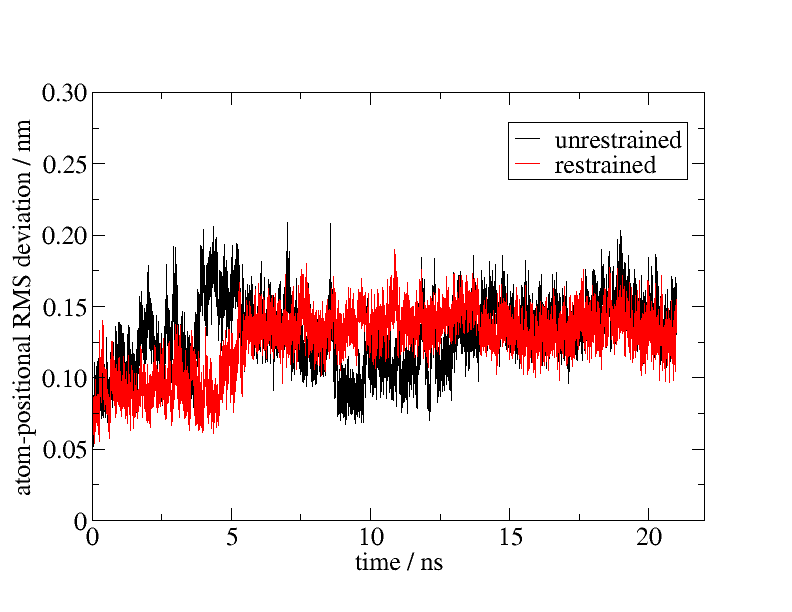
\includegraphics[scale=.3]{../04_tutorial_01/figures/GB3_RMSD}
\caption{Backbone atom-positional root-mean-square deviation (RMSD) of GB3 with respect to the final structure of the equilibration simulation.}
\label{GB3_rmsd}
\end{figure}

\begin{figure}[H]
\centering
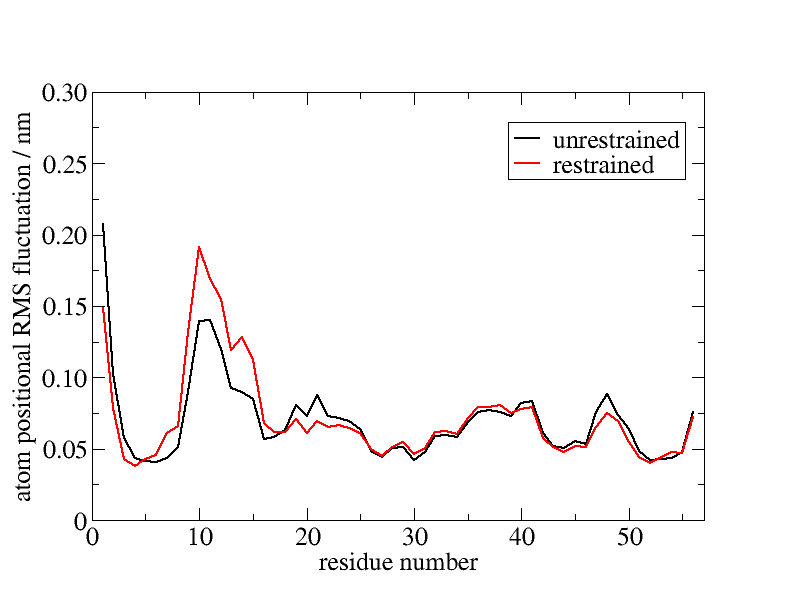
\includegraphics[scale=.3]{../04_tutorial_01/figures/GB3_RMSF}
\caption{Backbone N atom-positional root-mean-square fluctuation (RMSF) of GB3.}
\label{GB3_rmsf}
\end{figure}

\begin{figure}[H]
\centering
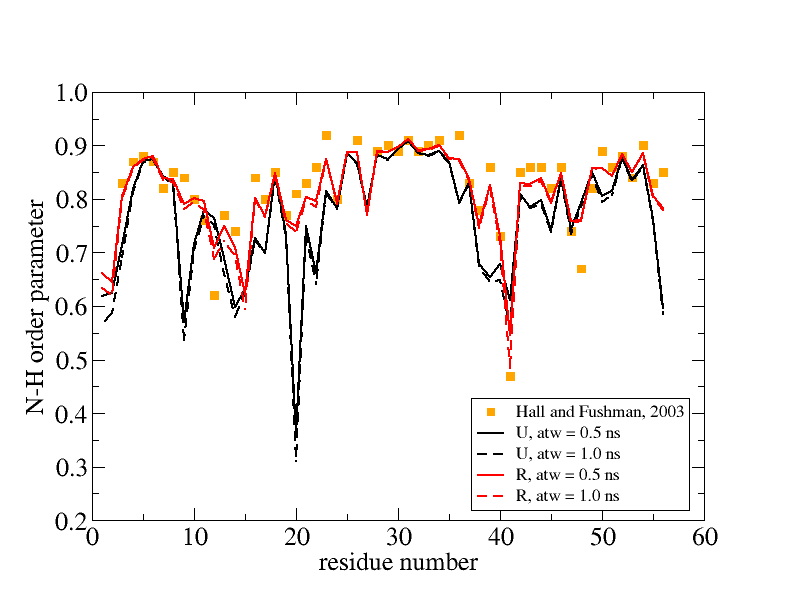
\includegraphics[scale=.3]{../04_tutorial_01/figures/GB3_S2}
\caption{Comparison of backbone N-H order parameters for protein GB3, determined from unrestrained (U) and restrained (R) MD simulations using different averaging time windows (atw) in the analysis. The experimentally derived order parameters used for restraining were taken from the work of Hall and Fushman ~\cite{Hall_2003} (anisotropic model).}
\label{GB3_S2}
\end{figure}








